\documentclass[margin=5pt]{standalone}

\usepackage{
	,multirow
	,makecell
	,bigstrut
	,booktabs
}

\usepackage{tikz}
\usetikzlibrary{arrows}

% arara: pdflatex
% arara: latexmk: { clean: partial }
\begin{document}
\begin{tabular}{ *{6}{c} }
\toprule
	Graph & Situation & EV.diff. & Real.diff. & Best response & \# of obs. \\
\midrule
	\multirowcell{2}[-2\bigstrutjot]{
		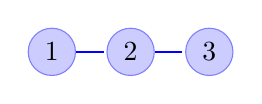
\begin{tikzpicture}
			\tikzstyle{player} = [
				circle, draw = blue!50, fill = blue!20,
				inner sep = 0pt, minimum size = 6mm
			]
			\tikzstyle{line}=[-,draw=blue,shorten >=1pt,>=stealth',semithick]
			\node[player] (1) at (0,0) {$1$};
			\node[player] (2) at +(0: 1) {$2$};
			\node[player] (3) at +(0: 2) {$3$};
			\draw (1) to (2) [line];
			\draw (2) to (3) [line];
		\end{tikzpicture}
	}
		& 1 (3) \(\rightarrow\) 2 & 4 & 3.7 & 0.854 & 151 \bigstrut \\
		& 2 \(\rightarrow\) 1 (3) & -12 & -12 & 0.948 & 77 \bigstrut \\
\cmidrule{2-6}
	\raisebox{-0.45\height}{
		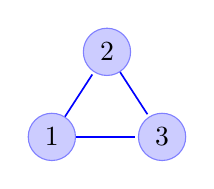
\begin{tikzpicture}
			\tikzstyle{player} = [
				circle, draw = blue!50, fill = blue!20,
				inner sep = 0pt, minimum size = 6mm
			]
			\tikzstyle{line}=[-,draw=blue,shorten >=1pt,>=stealth',semithick]
			\node[player] (1) at (0,0) {$1$};
			\node[player] (2) at (0.7, 1.08) {$2$};
			\node[player] (3) at (1.4, 0) {$3$};
			\draw (1) to (2) [line];
			\draw (2) to (3) [line];
			\draw (1) to (3) [line];
		\end{tikzpicture}
	}
		& 2 (3) \(\rightarrow\) 1 & 4 & 2.67 & 0.24 & 25 \bigstrut \\
	\cmidrule{2-6}
	\multirowcell{5}[-5\bigstrutjot]{{
		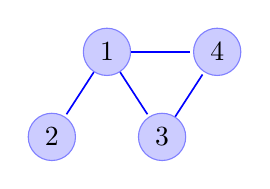
\begin{tikzpicture}
			\tikzstyle{player}= [
				circle, draw = blue!50, fill = blue!20,
				inner sep = 0pt, minimum size = 6mm
			]
			\tikzstyle{line}=[-,draw=blue,shorten >=1pt,>=stealth',semithick]
			\node[player] (1) at (0,0) {$1$};
			\node[player] (2) at (-0.7, -1.08) {$2$};
			\node[player] (3) at (0.7, -1.08) {$3$};
			\node[player] (4) at (1.4, 0) {$4$};
			\draw (1) to (2) [line];
			\draw (1) to (3) [line];
			\draw (1) to (4) [line];
			\draw (3) to (4) [line];
		\end{tikzpicture}
		}
	}
		& 2 \(\rightarrow\) 1 & -1.33 & 0.8 & 0.39 & 41 \bigstrut \\
		& 3 (4) \(\rightarrow\) 1 & 4 & 4.17 & 0.889 & 27 \bigstrut \\
		& 3 (4) \(\rightarrow\) 4 (3) & -4.7 & -6.33 & 0.676 & 37 \bigstrut \\
		& 1 \(\rightarrow\) 3 (4) & 4 & 4.25 & 0.5 & 32 \bigstrut \\
		& 1 \(\rightarrow\) 2 & -12 & -12 & 1 & 13 \bigstrut \\
	\bottomrule
\end{tabular}
\end{document}
